\section{Applications}\label{sec:examples}

We now explore the properties of \skye\ and compare it with PC EOS and HELM EOS.
When we refer to PC and HELM in the following we mean the MESA implementation
of each.  For PC this is based on source code made available by
A.~Potekhin.  It has been modified during its incorporation into MESA,
but not in ways that intentionally affect its results except for a
numerical blurring of the Coulomb phase transition. Likewise, the original source code of HELM
has been modified during its incorporation into MESA. Examples of such modifications include
providing third derivatives of the Helmholtz free energy and second derivatives
of the electron chemical potential,
using more accurate quadrature summations for derivatives of the Fermi-Dirac functions
when forming derivatives of the Helmholtz free energy \citep{gong_2001_aa},
supplying denser tables of the Helmholtz free energy and eight of its partial derivatives
(100 point per decade grid densities in $\rho$ and $T$), 
adding controls to activate or deactivate the pieces of physics in HELM, 
and deploying CR-LIBM \citep{CR-LIBM} for an efficient and proven correctly-rounded mathematical library
to ensure bit-for-bit identical results across platforms.

\subsection{Derivative Quality}

Figure~\ref{fig:dlnPgas_dlnRho} shows the relative difference between the reported derivative $\partial \ln p_{\rm gas}/\partial \ln \rho|_T$ and an iteratively acquired high-precision numerical derivative \citep[e.g.,][]{ridders_1982_aa,press_1992_aa} for each of \skye, HELM and PC.
Here $p_{\rm gas}$ is the total pressure minus radiation pressure.
For HELM and \skye\ we used the directly reported partial derivative while for PC we used $\partial \ln p_{\rm gas}/\partial \ln \rho|_T = \chi_\rho$.

Both \skye\ and HELM produce high-quality derivatives, better than one part in $10^{8}$, over much of the $\rho-T$ plane.
This is because \skye\ uses automatic differentiation on the analytic portion of the free energy and both \skye\ and HELM use spline partial derivatives on the tabulated ideal electron-positron free energy, so the quality of derivatives of thermodynamic quantities in these equations of state is limited only by the precision of floating-point arithmetic.
The PC derivative quality is somewhat lower than this primarily because of an internal redefinition of the density which occurs in the code but which is not propagated through the subsequent derivatives.

The grid structure in the derivative quality is set by the spacing of the HELM ideal electron-positron free energy table, on which both \skye\ and HELM rely.
At high temperatures above $10^9\,\mathrm{K}$ the system becomes dominated by electron-positron pairs and so nearly independent of the $\rho$.
The derivatives are then pushed towards the limits of floating point precision, degrading their quality.

The feature in \skye\ and PC at intermediate densities ($\rho \sim 1\,\mathrm{g\,cm^{-3}}$) and low temperatures ($T < 10^5\,\mathrm{K}$) results from negative pressures caused by the assumption of a fully ionized free energy in a region that should form bound states,
indicating that these equations of state are not valid in that limit.

\begin{figure}
	\centering
	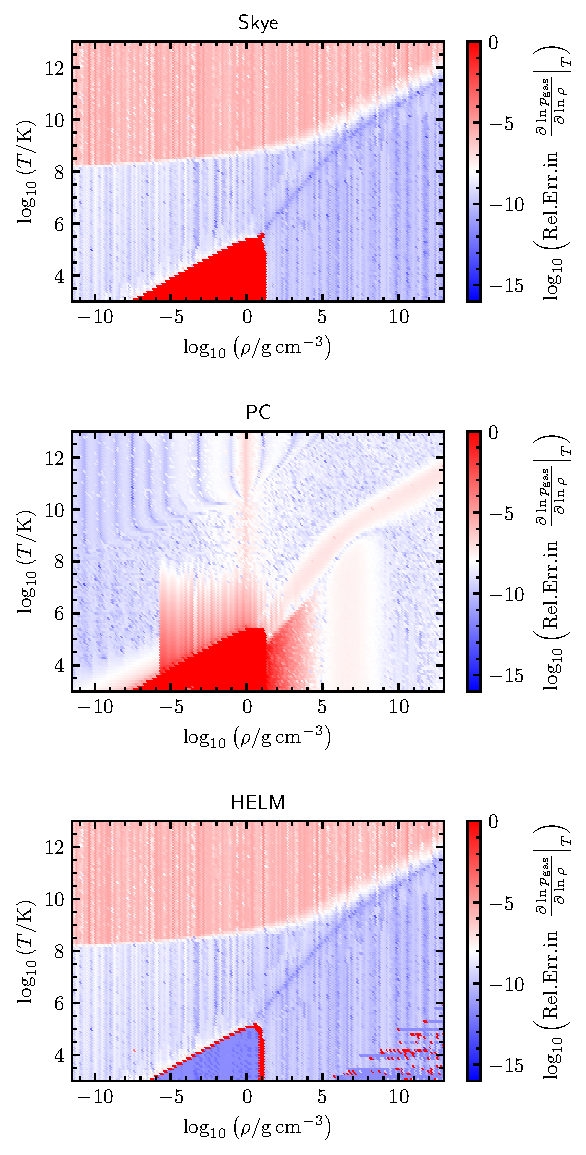
\includegraphics[width=0.45\textwidth]{dfridr_lnPgas_lnRho.pdf}
	\caption{The logarithm of the relative difference between $\partial \ln p_{\rm gas}/\partial \ln \rho|_T$ and a finite difference approximation to the same is shown as a function of $T$ and $\rho$ for each of \skye, PC, and HELM for an equal-mass fraction mixture of $^{12}\mathrm{C}$ and $^{16}\mathrm{O}$. The feature in \skye\ and PC at intermediate densities and low temperatures results from negative pressures caused by the assumption of a fully ionized free energy in a region that should form bound states, indicating that these EOSes are not valid in that limit.}
	\label{fig:dlnPgas_dlnRho}
\end{figure}

In general the quality of derivatives degrades as we look to higher orders because there is more room for precision issues.
Figure~\ref{fig:dChi_dlnRho} shows the relative difference between the reported derivative $\partial \chi_T/\partial \ln \rho|_T = \partial^2 \ln p / \partial \ln \rho\,\partial \ln T$ and an iteratively acquired high-precision numerical derivative for \skye\ and HELM.
Once more at high temperatures above $10^9\,\mathrm{K}$ the system becomes dominated by electron-positron pairs and so nearly independent of the $\rho$.
The derivatives in \skye\ and HELM are then pushed towards the limits of floating point precision, degrading their quality.

$\partial \chi_T/\partial \ln \rho|_T$ is not reported natively by PC so we could not include PC in this comparison.
Because MESA requires this derivative, when PC is used in MESA this derivative is estimated using finite differences in $\ln \rho$.  This results in derivatives that are accurate at only around the $10^{-2}$ level, which was often a bottleneck in stellar evolution calculations.

\begin{figure}
	\centering
	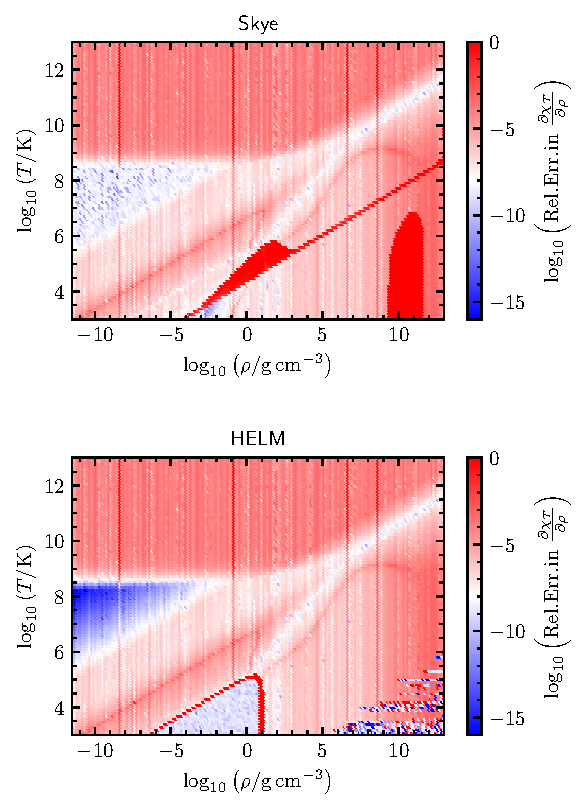
\includegraphics[width=0.45\textwidth]{dfridr_chiT_rho.pdf}
	\caption{The logarithm of the relative difference between $\partial \chi_T/\partial \ln \rho|_T$ a finite difference approximation to the same is shown as a function of $T$ and $\rho$ for \skye\ and HELM for an equal-mass fraction mixture of $^{12}\mathrm{C}$ and $^{16}\mathrm{O}$.}
	\label{fig:dChi_dlnRho}
\end{figure}

\subsection{Thermodynamic Consistency}

The first law of thermodynamics is an exact differential and thus implies several consistency relations between the different thermodynamic quantities.
These are~\citep[][see their Appendix A.1.3]{Timmes2000,Paxton2019}
\begin{align}
	\mathrm{dpe} \equiv \frac{\rho^2}{p}\left.\frac{\partial e}{\partial \rho}\right|_{T,\{y_j\}} + \frac{T}{p}\left.\frac{\partial p}{\partial T}\right|_{\rho,\{y_j\}} - 1 &= 0\\
	\mathrm{dse} \equiv T\frac{\partial s/\partial T|_{\rho,\{y_j\}}}{\partial e/\partial T|_{\rho,\{y_j\}}} - 1 &= 0\\
	\mathrm{dsp} \equiv -\rho^2\frac{\partial s/\partial \rho|_{T,\{y_j\}}}{\partial p/\partial T|_{\rho,\{y_j\}}} - 1 &= 0.
\end{align}
If these relations are not satisfied an equation of state is thermodynamically inconsistent.
For simulations of physical scenarios this can result in artificial generation or loss of energy or entropy or incorrect conversion between these and mechanical work.
Moreover thermodynamic inconsistency means that different forms of the same physical equations are not even mathematically identical.
For instance, neglecting changes in composition, in stellar evolution the equation of local energy conservation is often written as~\citep{Paxton2015}
\begin{align}
	\frac{de}{dt} - \frac{p}{\rho}\frac{d\ln \rho}{dt} = T \frac{ds}{dt},
\end{align}
or alternatively as
\begin{align}
	c_p T \left[(1-\nabla_{\rm ad} \chi_T) \frac{d\ln T}{dt} - \nabla_{\rm ad} \chi_\rho \frac{d\ln \rho}{dt}\right] = T \frac{ds}{dt}.
\end{align}
For numerical reasons it is often preferable to use one form over another, but these forms are only mathematically equivalent to the extent that the EOS is thermodynamically consistent.

\begin{figure}
	\centering
	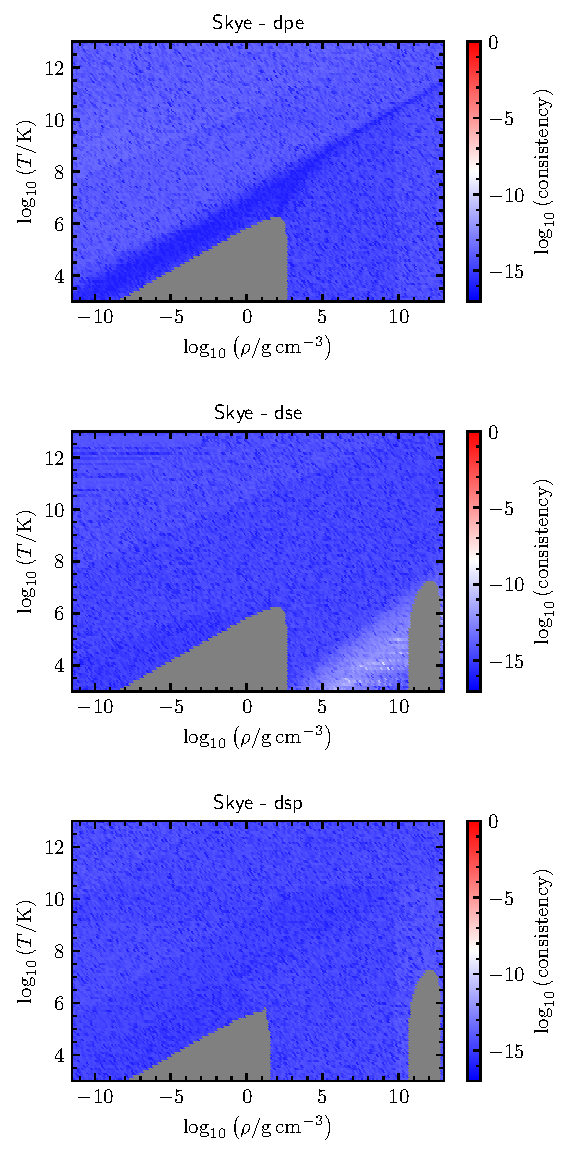
\includegraphics[width=0.45\textwidth]{consistency.pdf}
	\caption{The thermodynamic consistency measures $\mathrm{dpe}$, $\mathrm{dse}$, and  $\mathrm{dsp}$ are shown for \skye\ on a logarithmic scale for an equal-mass fraction mixture of $^{16}\mathrm{O}$ and $^{20}\mathrm{Ne}$. Grey indicates regions where the result is NaN due to negative reported entropy, energy, or pressure (solid regions) resulting in undefined logarithms in intermediate steps of the calculation. The feature at intermediate densities and low temperatures indicates negative pressures caused by our assumption of a fully ionized free energy in a region that should form bound states, indicating that \skye\ is not valid in that limit.}
	\label{fig:consistency}
\end{figure}

Figure~\ref{fig:consistency} shows the quantities $\mathrm{dpe}$,  $\mathrm{dse}$, and  $\mathrm{dsp}$ from \skye\ as functions of $\rho$ and $T$ for an equal-mass fraction mixture of $^{16}\mathrm{O}$ and $^{20}\mathrm{Ne}$.
Because \skye\ is derived from a free energy formalism it is thermodynamically consistent to the limits of floating-point precision.

Note that this high degree of consistency should not be confused with physical accuracy.
\skye\ returns \emph{numerically accurate} partial derivatives and thermodynamically consistent quantities, but this is not the same as \emph{physical} accuracy, which is a matter of how well the input physics matches Nature.


\subsection{Crystallization Curves}
\label{sec:ccurve}

We demonstrate where and how crystallization occurs in \skye\ by first
considering a pure $^{12}\rm C$ plasma at
$\rho=10^7\mathrm{g\,cm^{-3}}$.  Figure~\ref{fig:phase_OCP} shows the
location of crystallization and how that depends on which terms are
included in the free energy.\footnote{We can ignore any terms in the
  free energy that are not phase-dependent.}  The dotted line shows
the result of considering only the classical OCP free energy, which we
achieve by artificially forcing $\eta \to 0$ and deactivating the
screening terms.  This illustrates that crystallization is centered at
the established value of $\Gamma \approx 175$
\citep[e.g.,][and references therein]{PhysRevE.62.8554} and occurs over an an interval of
width $\Delta \Gamma \approx 10$ due to the blur described in
Section~\ref{sec:thermo}.  Including quantum corrections causes a
small shift ($\delta \Gamma \lesssim 1$) to higher values of $\Gamma$.
Adding screening results in much larger shift
($\delta \Gamma \approx 7$) towards lower values of $\Gamma$.%
\footnote{The size of this shift is larger than is shown in
  Figure 7 of \citet{PhysRevE.62.8554}. That calculation was done without quantum effects
  and used the fit from \citet{Yakovlev1989} for screening in the liquid regime instead of using Equation~(19) in \citet{PhysRevE.62.8554}.  The values of $f_{\rm ie}$ according to the two expressions are very close: the difference is $< 2$\%.  However, this difference in the screening correction is sufficient to noticeably affect the $\Gamma$ at which crystallization occurs, highlighting the sensitivity of the liquid/solid phase transition in Coulomb plasmas to tiny details in the free energy.}

\begin{figure}
	\centering
	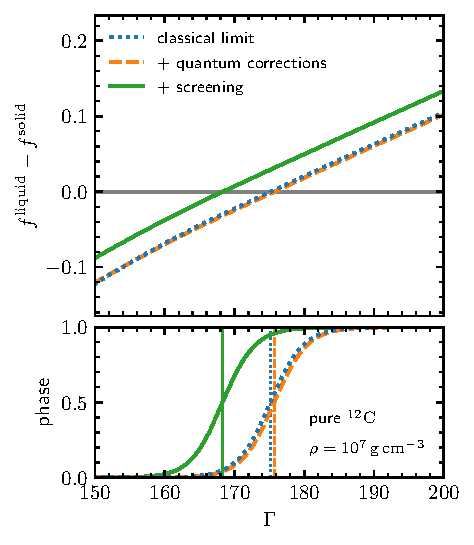
\includegraphics[width=0.45\textwidth]{gamma_crit.pdf}
	\caption{The liquid-solid free energy difference (top panel) and phase $\phi$ (bottom panel) as a function of $\Gamma$ for pure $^{12}\rm C$ plasma at $\rho=10^7\mathrm{g\,cm^{-3}}$.  We show the effects of different terms in the free energy by first showing the result in the classical limit (forcing $\eta \to 0$), then adding quantum effects, and finally including screening corrections.}
	\label{fig:phase_OCP}
\end{figure}


\skye\ determines the phase (solid/crystalline or liquid) self-consistently via free energy minimization, so it can model the effects of varying composition on melting temperature.
Figure~\ref{fig:phase_PC13} shows the phase as a function of temperature and composition in a $^{12}{\rm C}$-$^{16}{\rm O}$ mixture.
The x-axis, $x_{\rm O}$, is the $^{16}\rm O$ number fraction.  The y-axis, $T/T_{\rm m,C}$, is the ratio of the temperature to the melting temperature of a pure $^{12}\rm C$ plasma.
%
Because $\phi$ is a smoothed measure of the phase it takes a non-zero width to transition from $\phi \approx 0$ to $\phi \approx 1$.

The work of \citet{Blouin2020}, which adopts a Gibbs–Duhem integration technique coupled to Monte Carlo simulations, provides a useful point of comparison.
%
Their phase curve is calculated at $P = 10^{24}\,\mathrm{erg\,cm^{-3}}$ and so we calculate the Skye phase at $\rho=10^7\,\mathrm{g\,cm^{-3}}$ which corresponds to a similar pressure of $P \approx 8 \times 10^{23}\,\mathrm{erg\,cm^{-3}}$.
In Figure~\ref{fig:phase_PC13}, we show the \citet{Blouin2020} liquidus and solidus.
The reference melting temperature used for the \citet{Blouin2020} liquidus and solidus curves is the $T_{\rm m,C}$ value from \citet{Blouin2020}, which differs from the Skye value.
Recall Skye does not  consider phase separation, so it produces a single (blurred) transition line.

\begin{figure}
	\centering
	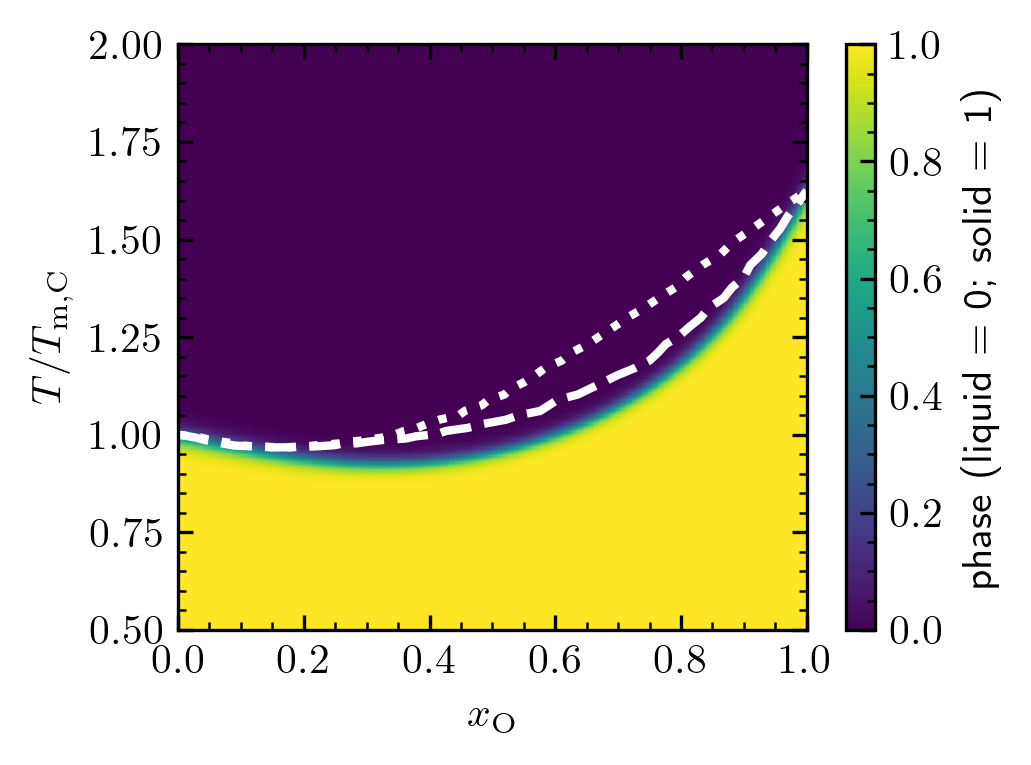
\includegraphics[width=0.45\textwidth]{PC13_phase_curve.png}
	\caption{The phase $\phi$ as a function of the ratio of the temperature to the melting temperature of a pure $^{12}\rm C$ plasma, $T/T_{\rm m,C}$, and $^{16}\rm O$ number fraction, $x_{\rm O}$, at fixed density $\rho=10^7\mathrm{g\,cm^{-3}}$ for a mixture of $^{12}\rm C$ and $^{16}\rm O$.  The white lines are the liquidus (dotted) and solidus (dashed) from \citet{Blouin2020}.}
	\label{fig:phase_PC13}
\end{figure}

As an example of how simple it is to swap out individual components in
the \skye\ framework, Figure~\ref{fig:phase_O93} shows the result
when we replace the (default) fit of \citet{2013A&A...550A..43P} for the solid mixing corrections with the form proposed by \citet{1993PhRvE..48.1344O}.
%
The \citet{2013A&A...550A..43P} form is in part motivated to overcome unphysical behavior%
\footnote{Specifically, \citet{2013A&A...550A..43P} note that the
  Ogata function is non-monotonic for fixed $x_2 < 0.5$ at $R > 2$.
  This is not simply a misbehaving fit.  The values in Table II of
  \citet{1993PhRvE..48.1344O} that are being fit show the same
  non-monotonic behavior.}
present in the \citet{1993PhRvE..48.1344O} fit at charge ratios $R > 2$,
though a C/O mixture ($R = 4/3$) is not in the troublesome regime.

The agreement shown in Figure~\ref{fig:phase_O93} between
\citet{Blouin2020} and Skye when using
\citet{1993PhRvE..48.1344O} is anticipated.
The results of \citet{Blouin2020} agree well with the results of
\citet{2010PhRvE..81c6107M}.  In turn, \skye\ resembles the
analytic-fit-based approach of \citet{2010PhRvE..81c6107M}, with the same extension from two-component to multi-component plasmas, and \citet{2010PhRvE..81c6107M} uses the \citet{1993PhRvE..48.1344O} formulation of the solid mixing free energy.


\begin{figure}
	\centering
	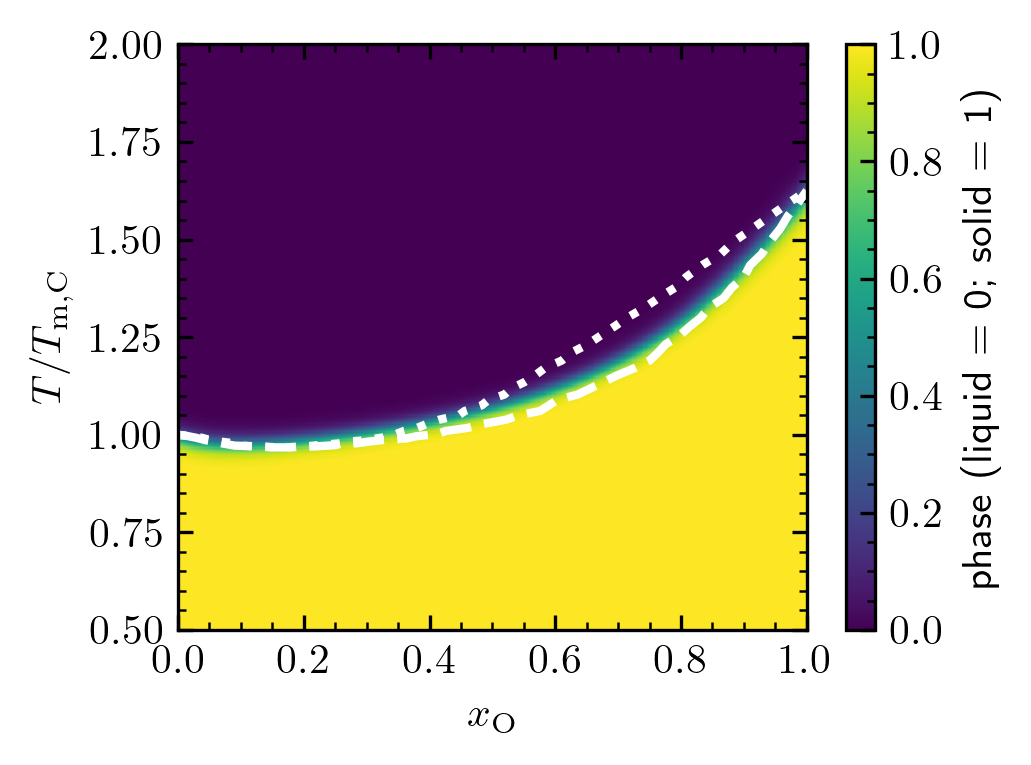
\includegraphics[width=0.45\textwidth]{Ogata93_phase_curve.png}
	\caption{Same as Figure~\ref{fig:phase_PC13}, except replacing the default solid mixing free energy from \citet{2013A&A...550A..43P} with the form proposed by \citet{1993PhRvE..48.1344O}.}
	\label{fig:phase_O93}
\end{figure}

\begin{figure}
  \centering
  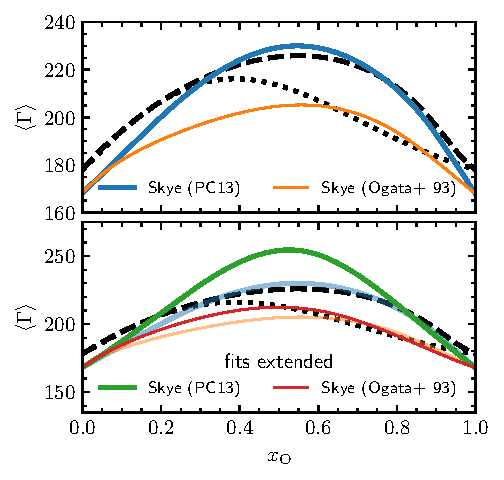
\includegraphics[width=0.45\textwidth]{phase_curve_gamma.pdf}
  \caption{Value of $\langle \Gamma \rangle$ corresponding to the center of the Skye phase transition
    ($\phi = 0.5$) as function of
    $^{16}\rm O$ number fraction $x_{\rm O}$ at fixed density
    $\rho=10^7\,\mathrm{g\,cm^{-3}}$ for a mixture of $^{12}\rm C$ and
    $^{16}\rm O$.
    The top panel compares the Skye results using the indicated solid mixing correction.
    The bottom panel shows the results when extending the limits of the solid and liquid fits (see text).
    The curves from the top panel are faintly shown for ease of comparison.
    In both panels, the black lines are the liquidus (dotted) and solidus (dashed) from \citet{Blouin2020}.}.\label{fig:phase_gamma}
\end{figure}


The results shown in Figures~\ref{fig:phase_PC13} and \ref{fig:phase_O93}
are summarized in the top panel of Figure~\ref{fig:phase_gamma} which plots the value
of the average Coulomb parameter $\langle \Gamma \rangle$ at
crystallization (defined as when $\phi = 0.5$) as a function of the
$^{16}\rm O$ number fraction.  For pure compositions, the Skye phase transition
occurs at a $\langle \Gamma \rangle$ value of about 10 less than \citet{Blouin2020},
primarily reflecting the screening corrections shown in Figure~\ref{fig:phase_OCP}.
The two approaches to the mixing corrections give significantly
different values for the phase transition in an equal (by number) mixture, with the \citet{1993PhRvE..48.1344O} form yielding
$\langle \Gamma \rangle \approx 205$ and the \citet{2013A&A...550A..43P} form yielding
$\langle \Gamma \rangle \approx 230$, with the \citet{Blouin2020} results intermediate.

%
% We see that, with the
% \citet{1993PhRvE..48.1344O} solid mixing corrections, crystallization in \skye\
% for a C/O binary mixture occurs within a $\langle \Gamma \rangle$ difference
% $\lesssim 20$ from the \citet{Blouin2020} liquidus for all
% compositions.
%
% The disagreement with the results of \citet{Blouin2020} caused by
% using the \citet{2013A&A...550A..43P} fit shown in
% Figures~\ref{fig:phase_PC13} and \ref{fig:phase_gamma} leads us to
% select the \citet{1993PhRvE..48.1344O} fit, especially since early
% applications of \skye\ will be in white dwarf cooling
% (Section~\ref{sec:cooling}).
% %
% At present, work focused on high-charge ratio mixtures ($R > 2$) might make a
% different selection.
% In particular the formula of~\citet{2013A&A...550A..43P} was constructed to match that of~\citet{2003CoPP...43..279D} at low charge ratios while exhibiting more physical behavior at high charge ratios.
%
Because the range of $\Gamma_j$ where both the liquid and solid free
energy fits are valid is small, for charge ratios greater than
$(\Gamma_{\rm max}^{\rm liquid}/\Gamma_{\rm min}^{\rm solid})^{1/2}
\approx 1.1$ one species or the other will typically be extrapolated
at the phase transition.  To illustrate this effect, the bottom panel
of Figure~\ref{fig:phase_gamma} shows a `fits extended' calculation
where we used $\Gamma_{\rm min}^{\rm solid}=100$ and
$\Gamma_{\rm max}^{\rm liquid} = 300$.  This shows that the
transition $\langle\Gamma\rangle$ may depend at the 10~per-cent level
on the choice of $\Gamma_{\rm max}^{\rm liquid}$ and $\Gamma_{\rm min}^{\rm solid}$.
%


The structure of \skye\ demands individual fits
that behave well over wide parameter ranges and a set of prescriptions
that can collectively work well together.
%
This is especially necessary for determining the location of the phase
transition, given the small relative difference between the liquid and
solid free energies.
%
We observe that Skye, at some unusual conditions, 
reports that material returns to the liquid state at sufficiently low
temperature as a result of the quantum corrections.
We discuss this behavior in Appendix~\ref{sec:quantum}.
%
We hope that the ease of
experimentation with \skye\ can help motivate improved fits for some
of the key quantities.


\subsection{Comparison with Other EOS}

We now compare various outputs from \skye, PC and HELM.
Figure~\ref{fig:gam1} shows the adiabatic index $\Gamma_1$ as a function of $\rho$ and $T$ for an equal-mass fraction mixture of $^{12}\mathrm{C}$ and $^{16}\mathrm{O}$.
The upper panel is for \skye\, the others show the signed logarithm of the relative difference between \skye\ and PC and HELM.
The outlined contour shows where $\Gamma_1 = 4/3$, signalling onset of the pair production instability.

At high temperatures and low densities ($T / 10^4 \,\mathrm{K} > (\rho/10^{-10}\,\mathrm{g\,cm^{-3}})^{1/3}$), \skye\ and HELM agree to better than one part in $10^5$, and both differ from PC by including positrons, which produce the feature that runs across the figure near $10^9\,\mathrm{K}$.

At lower temperatures and higher densities \skye\ and PC generally agree to better than one part in $10^{3}$.
The first exception is at intermediate densities and low temperatures, where both \skye\ and PC show artifacts caused by the assumption of a fully ionized free energy in a region that should form bound states, indicating these equations of state are not valid in that limit.
The other major difference is a series of scars at extreme densities and very low temperatures, which \skye\ inherits from the ideal electron-positron term in HELM.
In that regime computing thermodynamic quantities often requires subtracting very similar numbers, resulting in loss of precision.
The analytic fits PC uses for the ideal electron gas avoid this issue and produce smooth results there.

\begin{figure}
	\centering
	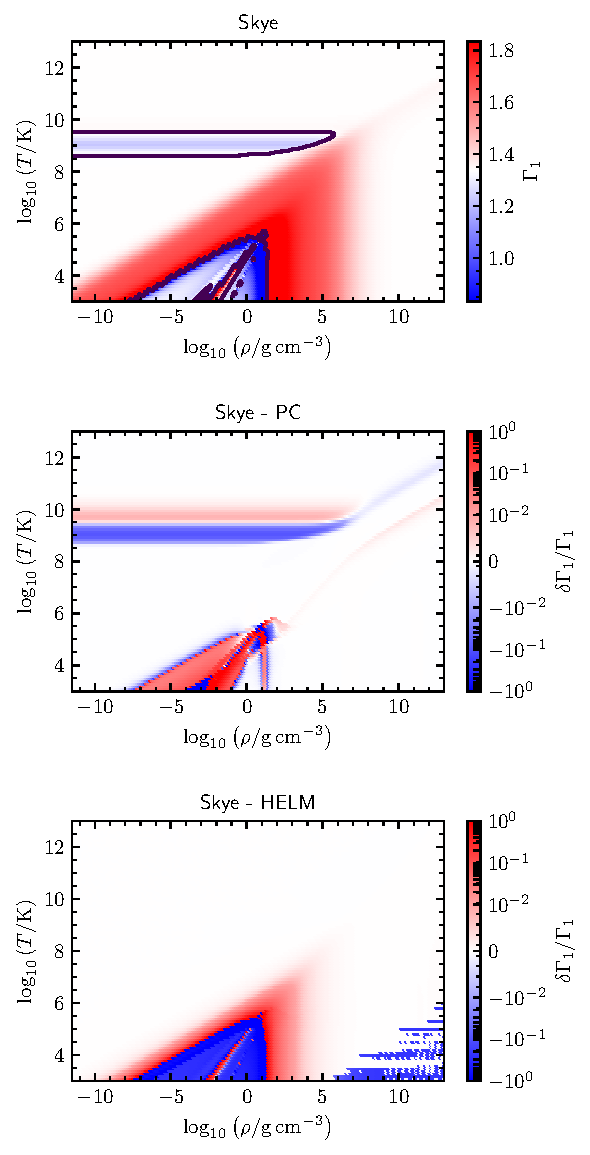
\includegraphics[width=0.45\textwidth]{gam1.pdf}
	\caption{The adiabatic index $\Gamma_1$ is shown as a function of temperature and density for each of \skye, PC, and HELM for an equal-mass fraction mixture of $^{12}\mathrm{C}$ and $^{16}\mathrm{O}$. The upper panel is for \skye\, the others show the relative difference between \skye\ and PC and HELM. The outlined contour shows where $\Gamma_1 = 4/3$, signalling onset of the pair production instability. Note that the outlined region in the bottom-right has $\Gamma_1 < 4/3$ because of precision issues in the ideal electron-positron tables and is not a sign of a physical instability.}
	\label{fig:gam1}
\end{figure}

Closely related to $\Gamma_1$, and of particular interest for asteroseismology, is the adiabatic temperature gradient $\nabla_{\rm ad}$.
Figure~\ref{fig:grada} shows $\nabla_{\rm ad}$ as a function of $\rho$ and $T$ for the same composition used in Figure~\ref{fig:gam1}.
Once more at high temperatures \skye\ and HELM agree at the $10^{-5}$ level, and both differ from PC by including positrons.
At lower temperatures we see an order-unity difference between \skye\ and PC which stretches along a line of nearly constant $\langle \Gamma \rangle$.
This difference is because PC places the phase transition at a fixed location in $\langle \Gamma \rangle$ while \skye\ determines the phase boundary from the input physics, which in this instance causes it to place the boundary at a slightly different $\langle \Gamma \rangle$.
The other major difference is that \skye\ again shows scars at very high density that come from loss of precision in the ideal electron-positron term in HELM.
Other than that region \skye\ and PC generally agree to better than one percent.

\begin{figure}
	\centering
	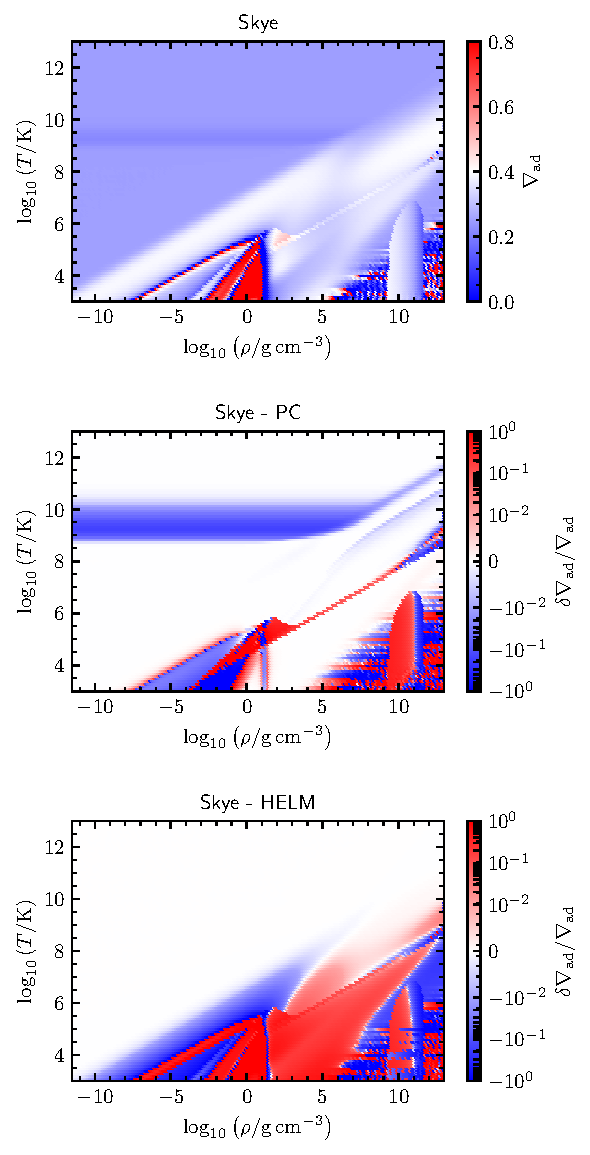
\includegraphics[width=0.45\textwidth]{grada.pdf}
	\caption{The adiabatic temperature gradient $\nabla_{\rm ad}$ is shown as a function of temperature and density for each of \skye, PC, and HELM for an equal-mass fraction mixture of $^{12}\mathrm{C}$ and $^{16}\mathrm{O}$. The upper panel is for \skye\, the others show the relative difference between \skye\ and PC and HELM.}
	\label{fig:grada}
\end{figure}

One of the most important quantities for white dwarf cooling models
(Section~\ref{sec:cooling}) is the specific heat.  Figure~\ref{fig:cv}
compares this quantity between PC and Skye for $^4\rm He$ and
$^{12}\rm C$.  In the case of $^{12}\rm C$, the agreement is generally
good, with some disagreement at the $\approx 10\%$ level around the
temperature of crystallization in the highest density line shown.
%
The dips near the location of the \skye\ phase transition are due to thermodynamic extrapolation and will be discussed in detail in Section~\ref{sec:cooling}.

% This plot is all of Cv (not just the ions), which I think is why one
% doesn't see the nice 3/2 limit in the highest T/lowest Rho.

In the case of $^{4}\rm He$, in coolest parts of the liquid regime, PC
produces specific heats that fall rapidly with decreasing temperature
and even become negative.  This reflects a difference in the assumed
physics.  This version of PC contains only the leading-order term in
the Wigner-Kirkwood expansion (which is pushed beyond its range
of validity of $\eta_j \la 1$ in these plots), while \skye\ includes the prescription of
\citet{2019MNRAS.490.5839B} which is valid up to $\eta_j \approx 12$.
At densities $\log_{10}(\rho/{\rm g\,cm^{-3}}) = $ 4, 5, and 6,
Figure~\ref{fig:cv} illustrates that the \citet{2019MNRAS.490.5839B}
prescription reasonably joins onto the $\propto T^3$ specific heat of the
Debye regime. For higher $^{4}\rm He$ densities, this join becomes
less smooth and by $\log_{10}(\rho/{\rm g\,cm^{-3}}) = 7$, \skye\ too
develops regions of negative specific heat, because by $\rho \ga 10^{7}\mathrm{g\,cm^{-3}}$ for Helium, $r_{s,j} \la 300$ which is beyond the validity of the fit by~\citet{2019MNRAS.490.5839B}.
Eliminating these features awaits future improvements in prescriptions for the free energy of the
quantum Coulomb liquid.

\begin{figure}
	\centering
	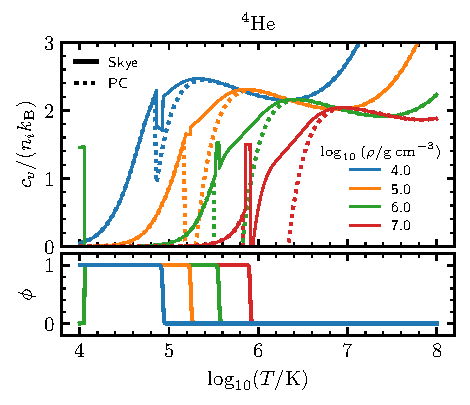
\includegraphics[width=0.45\textwidth]{cv_helium.pdf}
        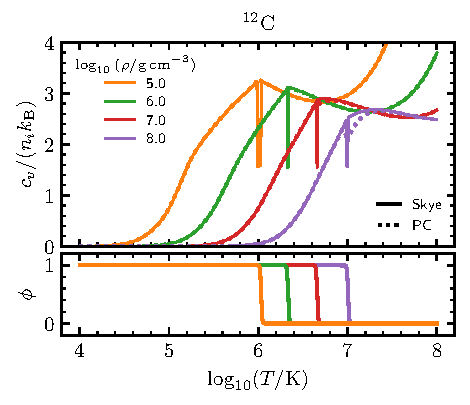
\includegraphics[width=0.45\textwidth]{cv_carbon.pdf}
	\caption{Comparison of specific heat between Skye and PC for $^4\rm He$ (top plot) and $^{12}\rm C$ (bottom plot) as function of temperature at an indicated set of densities.  Within each plot, the top panel shows the total specific heat at constant volume per ion for each of Skye and PC, while the bottom panel shows the Skye phase.}
	\label{fig:cv}
\end{figure}



\subsection{White Dwarf Cooling Curves} \label{sec:cooling}

We have computed white dwarf (WD) cooling curves using the Modules for
Experiments in Stellar Astrophysics~\citep[MESA;][]{Paxton2011,
  Paxton2013, Paxton2015, Paxton2018, Paxton2019} software
instrument. MESA uses a blend of several equations of state, and we
have configured the blend to use \skye\ in regions of high density or
temperature. 
Details of MESA, the blend, and other microphysics inputs are provided in Appendix~\ref{appen:mesa}.

Our example WD model is 0.6~$M_\odot$ with a C/O core and an initial
hydrogen layer mass of $5 \times 10^{-5}\ M_\odot$. This model is
based on the MESA test case \verb|wd_cool_0.6M| from MESA release
version 15140. Our cooling tracks begin when the model has a core
temperature of $\log_{10}(T_{\rm c}/K) = 7.8$ and luminosity of
1~$L_\odot$, and the WD cools until the core temperature reaches
$\log_{10}(T_{\rm c}/K) = 6.0$. We use the DA WD atmosphere tables of
\cite{Rohrmann12} as our outer boundary conditions for these WD
cooling models. The prior evolution of the WD progenitor model
included heavy element sedimentation so that the envelope is
stratified and the outer layers are composed of pure hydrogen, but for
simplicity we turn diffusion off for the cooling tracks calculated in
this paper. These models therefore do not include any cooling delay
associated with heating from sedimentation of $^{22}$Ne such as that
described in \cite{Paxton2018} and \cite{Bauer2020}. Instead, we focus
on cooling effects directly associated with EOS quantities such as
heat capacity and latent heat released by crystallization.

We run several versions of the WD cooling model described above, using
either \skye\ or the PC EOS in the high density regime
($\log_{10}(\rho/{\rm g\,cm^{-3}}) > 4$).
The PC EOS provides thermodynamics
for both liquid and solid states, with the location of the phase
transition a free parameter to be set by the user. As a baseline model
for comparison, we run the cooling WD with crystallization in PC set to
occur when the plasma reaches $\langle \Gamma \rangle = 230$, but with
no latent heat included in the model.
Previous WD cooling models using MESA have adopted this choice
of $\langle \Gamma \rangle = 230$ as a rough approximation of the C/O
phase curve in mixtures relevant for WD interiors (see
\cite{Bauer2020} for a recent example and further discussion).
We also run the WD cooling model using PC with crystallization
occurring at $\langle \Gamma \rangle = 175$ and $\langle \Gamma \rangle = 230$ with
the latent heat included in the models. 
When running with the PC EOS,
MESA models include the latent heat by taking the difference of entropy $s$
in the solid and liquid states, smoothed over a narrow range of
$\Gamma$ around the phase transition (e.g.\ in our case $228 < \Gamma < 232$
for crystallization at $\langle \Gamma \rangle = 230$). The latent
heating term is then constructed as
$\epsilon_{\rm latent} = -T (s_{\rm solid} - s_{\rm liquid})/\delta t$,
where $\delta t$ is the timestep. This latent heat is
included in the evolution as part of
$\epsilon_{\rm grav} \equiv -T ds/dt$ \citep{Paxton2018}. Finally, we
run the same WD cooling model with \skye\ as the EOS,
which includes the phase transition and the latent heat according
the phase curves shown in Figures~\ref{fig:phase_PC13}
and~\ref{fig:phase_gamma}.

\begin{figure}
  \centering
  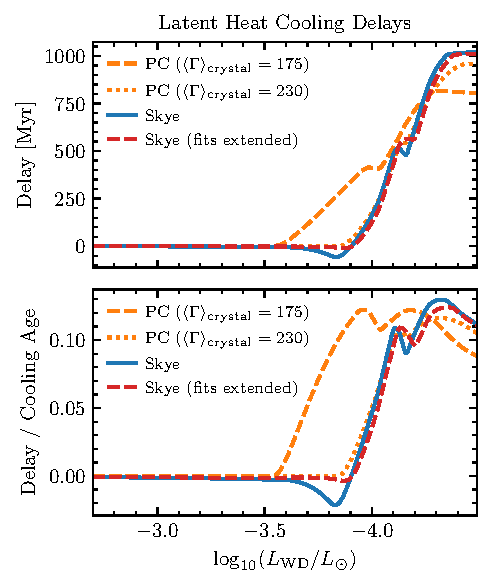
\includegraphics[width=0.45\textwidth]{CoolingDelay.pdf}
  \caption{Comparison of latent heat cooling delays for \skye\ and PC
    with crystallization occurring at two different values of
    $\langle \Gamma \rangle$. All delays are relative to a model run
    using the PC EOS with $\langle \Gamma \rangle_{\rm crystal} = 230$
    and no latent heat release.}
  \label{fig:delay}
\end{figure}

Figure~\ref{fig:delay} shows the cooling delay introduced into WD
models by latent heat from crystallization in models run with each of the PC EOS and \skye.
For \skye\ we performed two sets of calculations, one with the default extrapolation settings and another `fits extended' calculation where we used $\Gamma_{\rm min}^{\rm solid}=100$ and $\Gamma_{\rm max}^{\rm liquid} = 300$.

In general the \skye\ models agree well with the PC model run with
crystallization occurring at
$\langle \Gamma \rangle = 230$, which represents the previous state of
the art for WD cooling in MESA. Before crystallization begins around
$\log_{10}(L/L_\odot) = -3.8$, the lower panel of
Figure~\ref{fig:delay} also shows that the \skye\ WD models agree with
the overall cooling age of the PC model to better than 1\%.

The \skye\ models also agree well with each other despite the `fits extended' version applying the free energy fits over a wider range of temperatures.
The reason for this is that  \skye\ is thermodynamically consistent, so the overall cooling delay produced by the phase transition is insensitive to the choice of $\Gamma_{\rm max}^{\rm liquid}$ and $\Gamma_{\rm min}^{\rm solid}$.
To see this note that the entropy deep in the liquid phase (all $\Gamma_j < \Gamma_{\rm max}^{\rm liquid}$) is independent of the extrapolation process, and likewise for the entropy deep in the solid phase (all $\Gamma_j > \Gamma_{\rm min}^{\rm solid}$).
Hence, if the temperature varies little across the transition and extrapolation window then $\int T \partial s/\partial T dT$, counting the $\epsilon_{\rm latent}$ term, is nearly independent of the extrapolation limits.


\begin{figure}
  \centering
  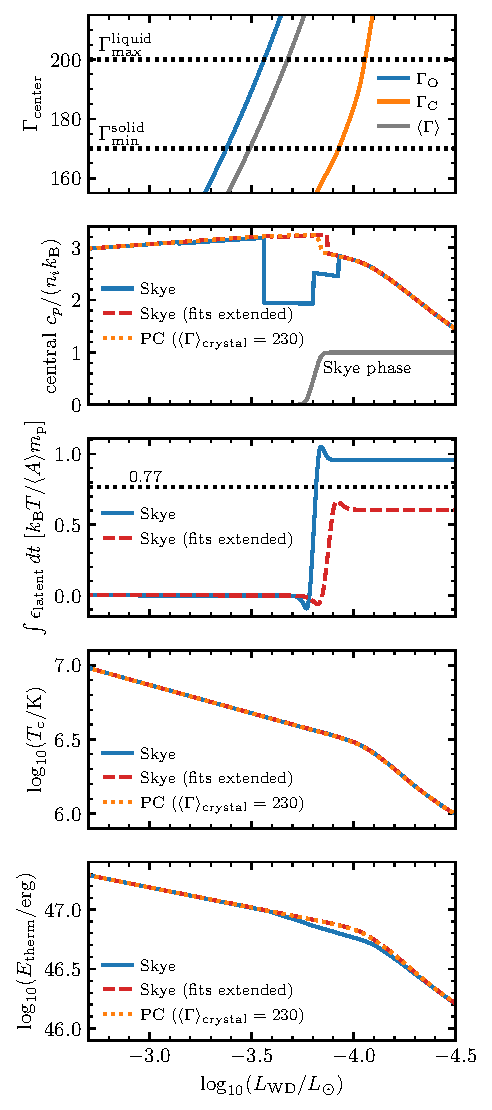
\includegraphics[width=0.45\textwidth]{LTc.pdf}
  \caption{Core thermodynamic properties as a function of luminosity
    for WD cooling models running on Skye and PC. In the second panel \skye\ phase refers to the quantity $\phi$ from equation~\eqref{eq:phi}.
  }
  \label{fig:LTc}
\end{figure}

Figure~\ref{fig:LTc} gives a comparison of the interior properties of
the WD cooling models from Skye and PC with crystallization at $\langle \Gamma \rangle = 230$.
As expected, the $L$--$T_{\rm c}$ relation agrees very well between Skye
and PC models, reflecting the similar input physics underlying these
two EOSs. Similarly, the total WD thermal content, defined as
$E_{\rm therm} \equiv \int c_p T \, dm$, agrees very well between the
two models.

The heat capacity $c_p$ in Figure~\ref{fig:LTc} shows some
disagreement in the region near the phase transition from liquid to solid.
The notch-like behavior in the \skye\ $c_p$ is a result of our thermodynamic extrapolation prescription (Section~\ref{sec:extrapolate}).
This is because the one-component plasma contribution to $\partial s/\partial T$ vanishes when we extrapolate, so the contribution to $c_v$ vanishes:
\begin{align}
	c_v &=  \left.\frac{\partial e}{\partial T}\right|_{\rho}\nonumber\\
	&= \left.\frac{\partial (F+Ts)}{\partial T}\right|_{\rho}\nonumber\\
	&= \left.\frac{\partial F}{\partial T}\right|_{\rho} + s + T\left.\frac{\partial s}{\partial T}\right|_{\rho}\nonumber\\
	&= T\left.\frac{\partial s}{\partial T}\right|_{\rho}.
\end{align}
Therefore, for any species at a $\Gamma_j$ where its free energy is being extrapolated, its OCP contribution to $c_v$ vanishes.
Because $c_p \sim c_v$, this causes a drop in $c_p$ as well.
Reading from left to right in the $c_p$ panel of Figure~\ref{fig:LTc}, the core begins in the liquid phase and initially no extrapolation is needed for the liquid phase free energy because $\Gamma_j < \Gamma_{\rm max}^{\rm liquid}$ for all species.
As the core cools, the $\Gamma_j$ rise.
The heat capacity falls sharply when $\Gamma_{^{16}\rm O}$ reaches $\Gamma_{\rm max}^{\rm liquid}$ because past that point we extrapolate the OCP free energy of $^{16}\rm O$.
The core continues cooling and then crystallizes at $\log L/L_\odot = -3.8$.
At this point the heat capacity is determined by the solid phase free energy.
Because  $\Gamma_{^{16}\rm O} > \Gamma_{\rm min}^{\rm solid}$, the OCP free energy of $^{16}\rm O$ is no longer extrapolated, but $\Gamma_{^{12}\rm C} < \Gamma_{\rm min}^{\rm solid}$ so the free energy of $^{12}\rm C$ is now extrapolated in the solid phase.
Finally, once $\log L/L_\odot = -3.9$, $\Gamma_{^{12}\rm C} > \Gamma_{\rm min}^{\rm solid}$ so we stop extrapolating the $^{12}\rm C$ free energy, causing a jump in $c_p$.
At this stage no species are extrapolated, and the heat capacity remains smooth for the rest of the run.

As before we note that because \skye\ is thermodynamically consistent the overall cooling delay is insensitive to the choice of limits for thermodynamic extrapolation and hence to these features in $c_p$.
So for instance in Figure~\ref{fig:LTc} extrapolation reduces $c_p$ near the phase transition relative to the `fits extended' version of \skye.
The third panel of Figure~\ref{fig:LTc} shows the total latent heat released in the core in terms of the thermal energy per ion at the temperature of crystallization, and we see that this is decreased for the `fits extended' version.
Thus the \emph{decrease} in $c_p$ is offset in the overall cooling calculating by an \emph{increase} in $\epsilon_{\rm latent}$, resulting in the regular and `fits extended' versions of \skye\ showing very similar cooling curves in Figure~\ref{fig:delay}.

In both the regular and `fits extended' versions of \skye\ we see that the overall magnitude of the latent heat is similar to the value of
$0.77 k_{\rm B}T/\langle A \rangle m_{\rm p}$ calculated by
\cite{Salaris2000}, which has often been adopted in recent studies of
WD cooling using other stellar evolution codes (e.g.,
\citealt{Camisassa2019}).
It is likewise similar to the results of~\citet{2013A&A...550A..43P}, who obtained an improved value of $0.75 k_\mathrm{B} T / A m_\mathrm{p}$ in the case of the one component plasma with the `rigid' electron backgroung and showed that the allowance for electron polarization/screening can lead to deviations of up to a factor of two from this value.

In our testing these sharp features in $c_p$ have not caused any convergence problems in MESA.
However, if this behavior is undesirable, $\Gamma_{\rm min}^{\rm solid}$ can be lowered and $\Gamma_{\rm max}^{\rm liquid}$ can be raised to ensure that, for any given composition, extrapolation is only used for the liquid phase when the system is solid, and vice versa, with the caveat that this risks using fitting formulas beyond the region in which they are known to be accurate.
This is what is shown in the `fits extended' curves in Figures~\ref{fig:delay} and~\ref{fig:LTc}, where we used $\Gamma_{\rm min}^{\rm solid}=100$ and $\Gamma_{\rm max}^{\rm liquid} = 300$.
Our hope is that future work on multi-component plasmas will provide a way to capture the behavior of, e.g., low-$\Gamma$ carbon in a multi-component solid.
This could take the form of e.g., fits for the two-component plasma free energy at the phase transition as a function of the charge ratio between the two species.

\begin{figure}
  \centering
  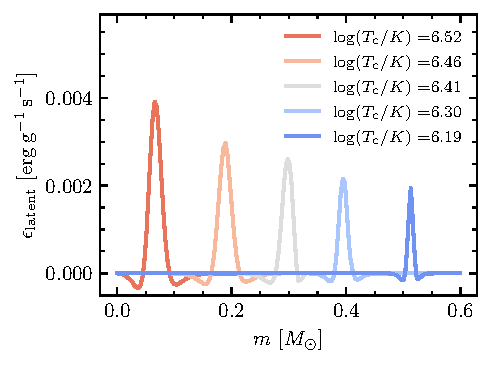
\includegraphics[width=0.45\textwidth]{Eps_latent.pdf}
  \caption{Evolution of the latent heating term from \skye\ as the WD
    model cools and the crystallization front moves from the center
    toward the surface.}
  \label{fig:eps_latent}
\end{figure}

\begin{figure}
  \centering
  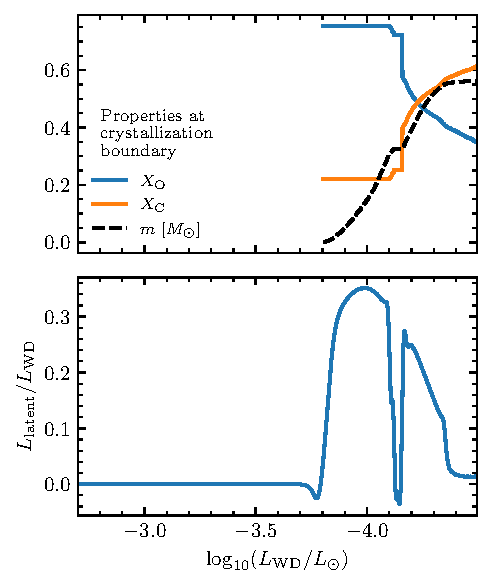
\includegraphics[width=0.45\textwidth]{L_latent.pdf}
  \caption{{\it Upper panel:} Curves showing the mass coordinate and
    composition of material at the crystallization boundary as a
    function of WD luminosity.
    {\it Lower panel:} Total luminosity from latent heating as a fraction of the
    WD luminosity, where $L_{\rm latent} \equiv \int \epsilon_{\rm latent} \, dm$.}
  \label{fig:l_latent}
\end{figure}

Figures~\ref{fig:eps_latent} and~\ref{fig:l_latent} show more details
about the latent heating term from Skye in our WD cooling model.
Figure~\ref{fig:eps_latent} shows how the blurred phase
transition distributes the latent heat in the WD interior as the
crystallization front moves outward while the WD cools. Integrating
these heating profiles over the entire WD gives a total latent heating
luminosity $L_{\rm latent}$, which is shown in Figure~\ref{fig:l_latent}.
The upper panel of that figure also shows the composition and mass
coordinate location of the crystallization boundary (defined as the
location where Skye phase = 0.5). We note that as the crystallization
front moves outward, there is a brief pause in crystallization and the
latent heating goes to zero when the front reaches a location where
the core composition becomes more carbon-rich. This location
corresponds to the outer edge of the former convective He-burning
core at the end of central He-burning, where C/O layers exterior to
this point were produced by subsequent He shell burning and therefore
have a different C/O composition than the interior homogeneous core.
This relatively carbon-rich layer has a lower crystallization
temperature than the adjacent C/O core interior to it, and so the core
temperature must cool further before crystallization resumes and the
latent heat returns.

\begin{figure}
  \centering
  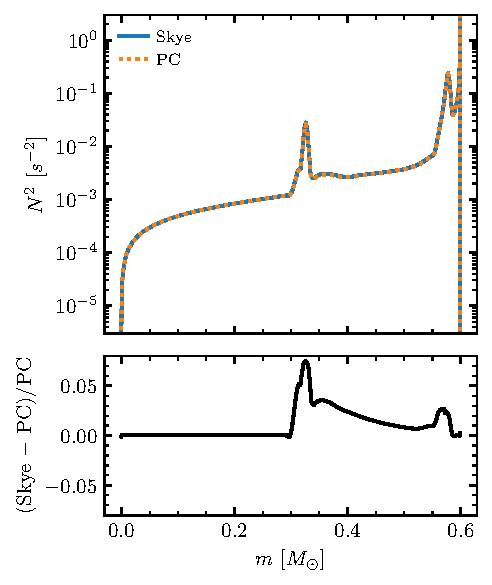
\includegraphics[width=0.45\textwidth]{BV.pdf}
  \caption{{\it Upper panel:} The \brvs\ frequency is shown as a function of mass coordinate for the \skye\ and PC WD models at a time when $\log T_{\rm c}/\mathrm{K} = 7.05$ and $T_{\rm eff} = 11,800\,\mathrm{K}$.  {\it Lower panel:} The relative difference between the two models is shown as a function of mass coordinate.}
  \label{fig:BV}
\end{figure}

Finally, Figure~\ref{fig:BV} shows the profile of the \brvs\ frequency for both the \skye\ and PC WD models, as well as the relative difference between the two.
The differences are generally of order a few percent.
For $m > 0.3 M_\odot$, there are differences in the composition gradient region.
These arise because \skye\ treats the density $\rho$ as the baryonic mass density whereas PC treats it as the physical mass density.
Either choice is valid, but neither is fully consistent with how \code{MESA} computes either the \brvs\ frequency or hydrostatic equilibrium, and these inconsistencies produce the differences we see for $m > 0.3 M_\odot$.

\section{Execution Efficiency}
\label{sec:speed}

\skye\ is designed to be fast enough to evaluate at runtime in stellar evolution calculations.
We benchmarked \skye, HELM, and PC on a single core of an Intel Core i9 (I9-9980HK) CPU running at 2.4GHz.
For this test PC was modified to use CR-LIBM for mathematical operations to ensure bit-for-bit identical results across platforms just like \skye\ and HELM.

We evaluated each EOS on a log-spaced grid in $\rho$ spanning $10^{-10}-10^{10}\,\mathrm{g\,cm^{-3}}$ with 600 points and in $T$ spanning $10^3-10^{10}\,\mathrm{K}$, with 500 points.
We require each EOS to return all of the quantities listed in Section~\ref{sec:thermo} except for the \skye-specific ones, as well as the partial derivatives of each of those quantities with respect to $\rho$ and $T$.
Because PC does not natively provide those derivatives, we use three calls of PC per point and then extract the additional derivatives with finite differences.

Averaged over all points in our grid, \skye\ takes $17\mu\mathrm{s}$ per call, PC takes $9\mu\mathrm{s}$ per call, and HELM takes $6\mu\mathrm{s}$ per call, where again we evaluate PC three times per call to produce the additional derivatives required by stellar evolution software instruments such as MESA.

As a second benchmark, we tracked the time spent in the MESA EOS module during the white dwarf cooling study from Section~\ref{sec:cooling}.
The EOS accounted for 10.5 per-cent of total run time when using PC, and 13.9 per-cent of total run time when using \skye.
This understates the difference between the two slightly because some of the time the stellar model is at a temperature and density where neither PC nor \skye\ are used, but shows that the runtime difference is minimal not only on a grid but also in practice in stellar evolution calculations.

\skye\ and PC have similar performance for several reasons:
\begin{enumerate}
	\item The physics that enters these equations of state is similar.
	\item Our automatic differentiation type is heavily optimized, and in many cases produces performance similar to hand-coded derivatives.
	\item The additional cost of determining higher-order derivatives with automatic differentiation happens to be very similar to the overhead of calling PC three times to obtain the same derivatives with finite differences.
	\item While \skye\ has to compute the non-ideal free energy twice to obtain phase information, this extra cost relative to PC is offset by the fact that \skye\ uses free energy tables for the ideal electron-positron contribution while PC computes this with more expensive fitting formulas.
\end{enumerate}
We determined (3) by producing a modified version of PC which produces higher-order derivatives using automatic differentiation rather than finite differences and found its performance to be similar to the unmodified PC.

HELM is much faster than either \skye\ or PC for three main reasons.
First, HELM uses an average composition characterized by the mean molecular weight and mean charge, 
rather than directly using the full composition vector $\{y_j\}$.
Second, the computationally expensive parts of HELM (a root-find for the electron chemical potential, 
high precision Fermi-Diac integrals, and nearly all operations involving division, exponentials, and power functions) are tabulated 
on a logically rectalinear array. Each call to HELM then consists of hash table lookups followed 
by calls to fast polynomial interpolation functions.
Third, thermodynamic information for neighboring points are located next to each other in physical memory. 
Ordered sweeps, such as from the surface of a stellar model to the center, 
will usually access data already loaded into the processor cache rather than having to access 
data from the slower main memory. This reduction in the time required to access
information from memory boosts the execution efficiency.


